\section{The experiment}

% ------------------------------------------------------------------------------
\begin{frame}
\frametitle{Agenda}
\tableofcontents[currentsection]
\end{frame}
% ------------------------------------------------------------------------------

% ------------------------------------------------------------------------------
\begin{frame}[fragile]
\frametitle{Repartition Join}
\begin{itemize}
  \item Equi-Join über 2 Relationen
  \item Mapper: wird jedes Tupel einmal weitergegeben oder ausgefiltert
  \item Partitioner: Modulo-Division des Schlüssel-HashWerts
\end{itemize}

\scriptsize{
\lstset{framexleftmargin=5mm, frame=shadowbox, rulesepcolor=\color{lightgray}}
\begin{lstlisting}
public void map(...) throws IOException 
{
    RelationTuple tuple = new RelationTuple(value);
    ...
    if (!filter.eval(tuple)) output.collect(outputKey, tuple);
}
\end{lstlisting}

\lstset{framexleftmargin=5mm, frame=shadowbox, rulesepcolor=\color{lightgray}}
\begin{lstlisting}
public int getPartition(RepartitionKey k, RelationTuple v, int ptns) 
{
    return Math.abs(k.getKey().hashCode() % ptns);
}
\end{lstlisting}
}
\end{frame}
% ------------------------------------------------------------------------------

% ------------------------------------------------------------------------------
\begin{frame}[fragile]
\frametitle{Repartition Join}
\begin{itemize}
  \item Sort:
  \begin{itemize} 
    \item primär nach Key 
    \item sekundär nach Relation ($L$ Relation kommt zuerst)
  \end{itemize}
  \item Reduce:
  \begin{itemize}
    \item alle $L$-Tupel zum aktuellen Schlüssel sammeln
    \item mit allen passenden $R$-Tupel kombinieren (kommen gleich danach)
  \end{itemize}
\end{itemize}
\end{frame}
% ------------------------------------------------------------------------------

% ------------------------------------------------------------------------------
\begin{frame}
\frametitle{TPCH Schema}
\begin{center}
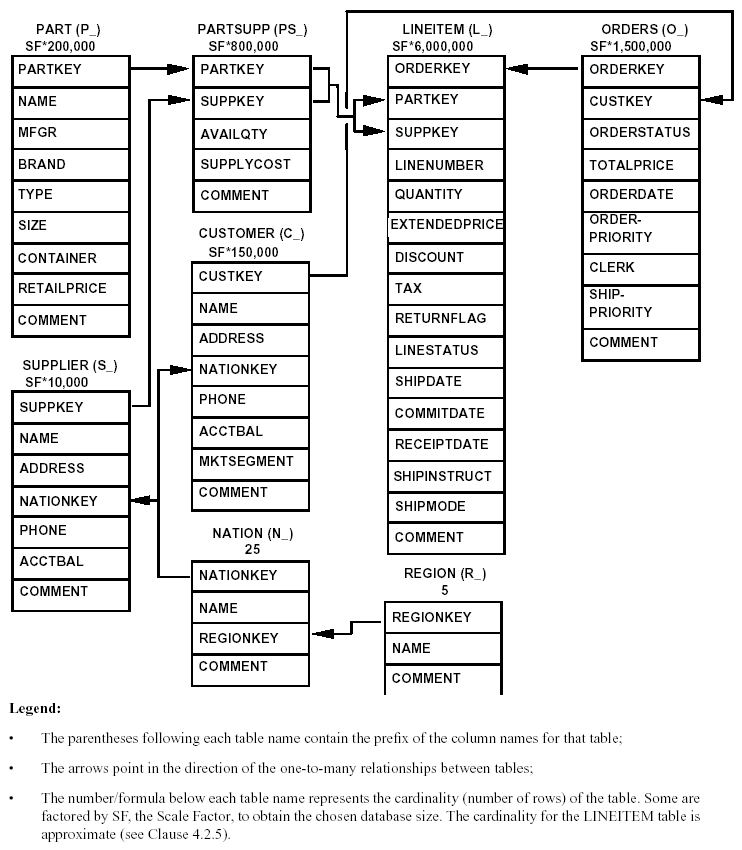
\includegraphics[width=.9\linewidth]{tpch-schema}
\end{center}
\end{frame}
% ------------------------------------------------------------------------------